\section{Results}\label{sec:results}

This section presents the testing results of the proposed solution.
First, hyper-parameters are tested in order to determine their reasonable values in subsection~\ref{subsec:hyper-parameters}.
Next, using these values, the results of performance tests are presented subsection~\ref{subsec:performance}.
Lastly, the best-obtained solutions are visualized in the section~\ref{subsec:visualization}.

\subsection{Hyper-parameters}\label{subsec:hyper-parameters}

\subsubsection*{Population size}

Population size is tested in order to determine a reasonable value called \textit{population scaling factor}.
This value determines the size of the population with respect to the instance size.
Thus, for instance, with size $N$ and scaling factor $k$, population size is determined as
$k \times N$.
This means that the population size is linear with respect to the instance size.

Results for two random instances can be seen in figure~\ref{fig:pop-size}.
From it, we can deduce that scaling factor $10$ does not allow
the population objective average to decrease to the levels comparable to scaling factors $50$ and $100$.
This might imply that the scaling factor $10$ is insufficient to represent knowledge gathered over time
in the genetic approach.
Also, researches in~\cite{goncalvesBiasedRandomkeyGenetic2015} solving UA-FLP using BRKGA
similarly obtained their best results for scaling factor $100$.

The conclusion is that using scaling factor between $50$ and $100$ is sufficient, with bias towards $100$
for obtaining better average objective performance.
However, increasing the scaling factor leads to slower computation speed as every population contains
more individuals for which genetic operators and reproductive plan must be computed.

\subsubsection*{Overlapping penalization constant}

It is not desirable to produce a solution where paintings overlap.
Thus, \textit{overlapping penalization constant} is used to penalize
individuals that represent such a solution.
How this constant is used inside the objective function is in equation~\ref{eq:objective}.

The optimal value where the penalization is strong enough
to uproot overlapping solutions from the population and, at the same time, low enough
to be at the same scale as other parts of the objective value are tested on four instances – random\_10, random\_20, cluster\_10, and cluster\_20.

Value tested for \textit{overlapping penalization constant} is proportional to the diagonal length of the layout to which paintings are placed.
Thus, if $w$ is width and $h$ is height of the layout, tested value is called $k$ which determines
\textit{overlapping penalization constant} as $k\sqrt{w^2 + h^2}$.

Results are in figure~\ref{fig:overlapping-random} for the two random instances and in figure~\ref{fig:overlapping-cluster} for two cluster instances.
From it, we can deduce that the optimal value for \textit{overlapping penalization constant} is between $1$ and $5$ times the length of the layout diagonal.

\afterpage{%
    \clearpage% Flush earlier floats (otherwise order might not be correct)
    \begin{landscape}% Landscape page
        \begin{figure}
            \centering
            \subfloat{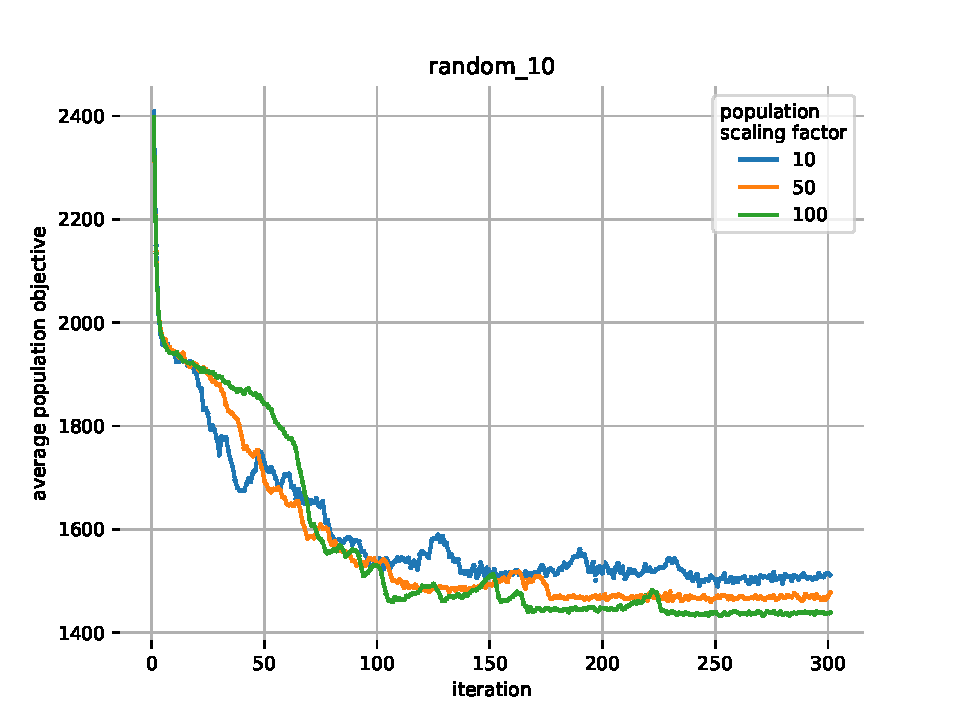
\includegraphics[width=0.8\textwidth]{pop_size_random_10}\label{subfig:pop-size-random-10}}
            \subfloat{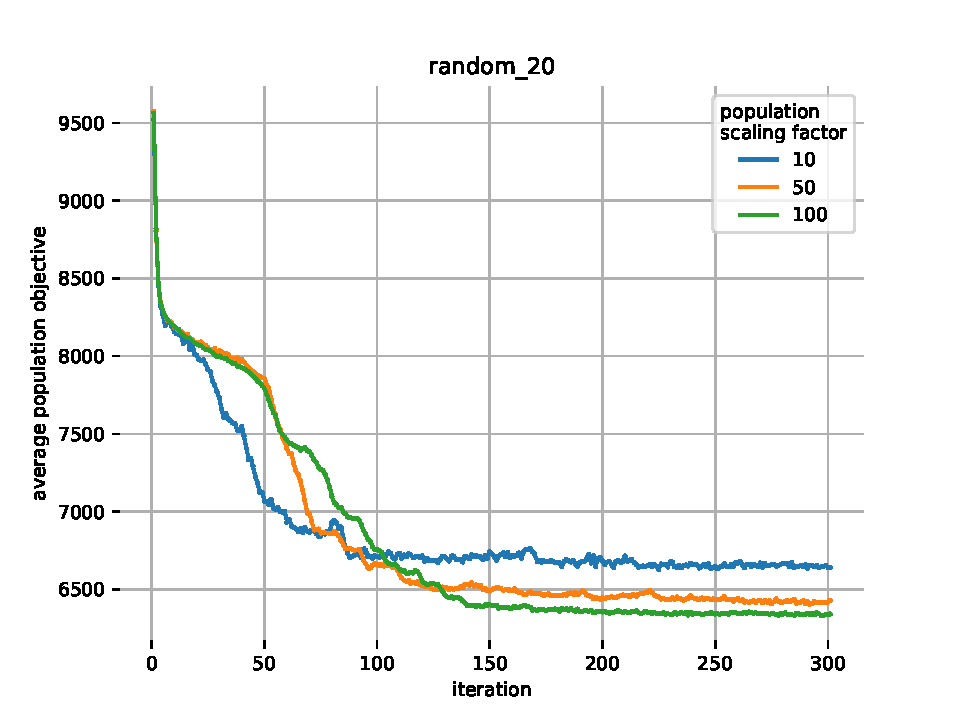
\includegraphics[width=0.8\textwidth]{pop_size_random_20}\label{subfig:pop-size-random-20}}
            \caption[Testing population scaling factor]{Testing population scaling factor at two random instances.}
            \label{fig:pop-size}%
        \end{figure}
    \end{landscape}
    \clearpage% Flush page
}

\subsection{Performance}\label{subsec:performance}

\afterpage{%
    \clearpage% Flush earlier floats (otherwise order might not be correct)
    \begin{landscape}% Landscape page
        \begin{figure}
            \centering
            \subfloat{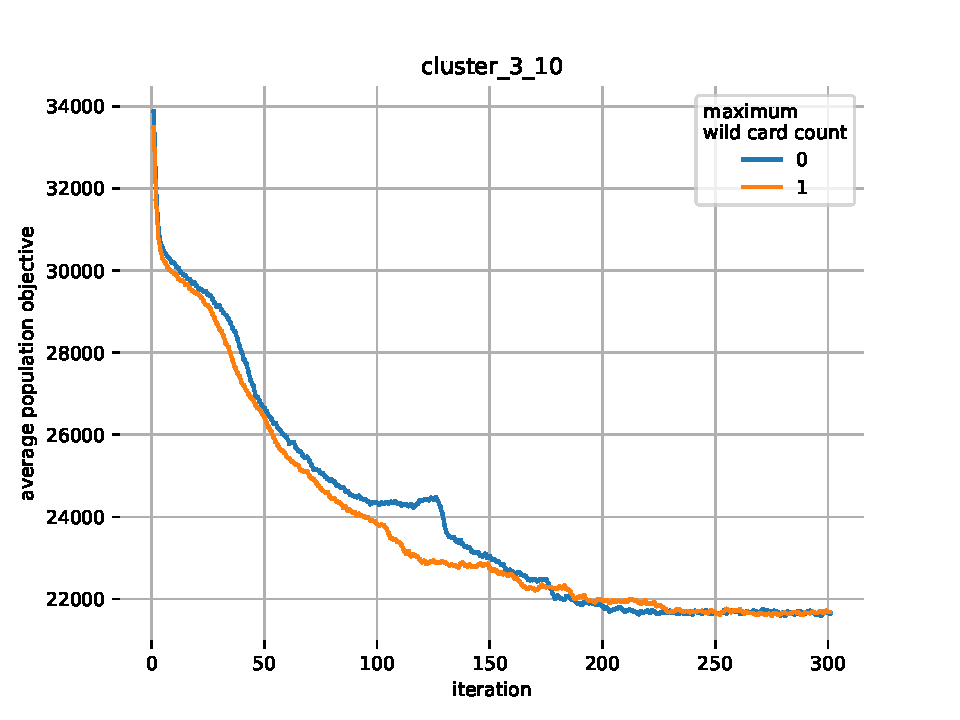
\includegraphics[width=0.8\textwidth]{cluster_3_10}\label{subfig:cluster-3-10}}
            \subfloat{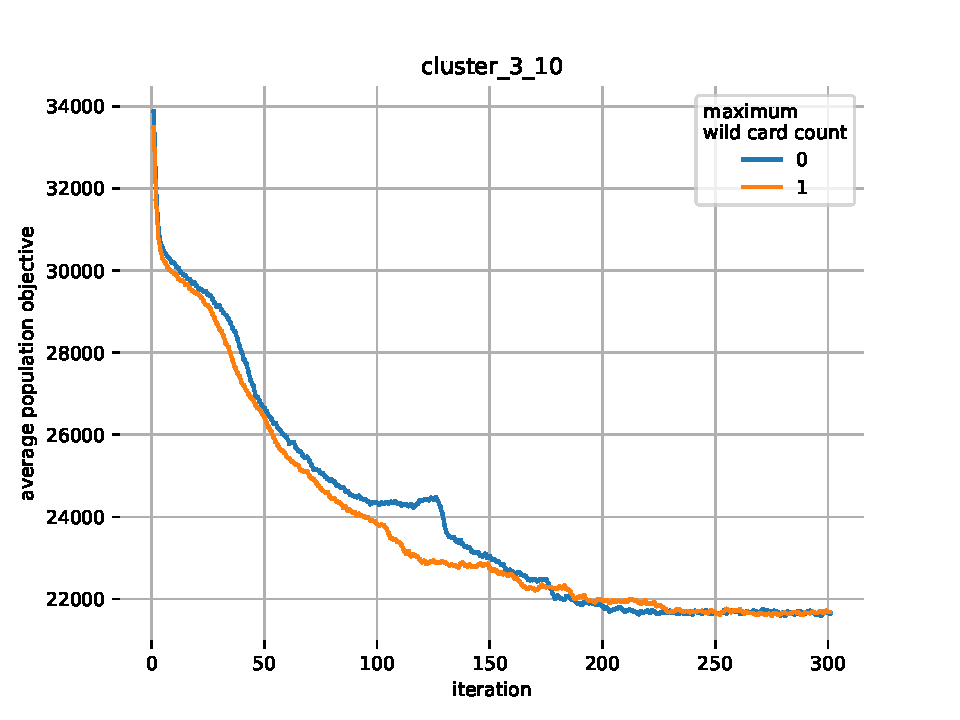
\includegraphics[width=0.8\textwidth]{cluster_3_10}\label{subfig:cluster-3-10}}
            \caption[Testing clustering dataset]{Testing clustering dataset performance with a different maximum wildcard count.}
            \label{fig:cluster}%
        \end{figure}
    \end{landscape}
    \clearpage% Flush page
}

\subsection{Visualization}\label{subsec:visualization}
